\documentclass[a4paper, 11pt]{article}
\usepackage[utf8]{inputenc}
\usepackage{amsmath}
\usepackage{graphicx}
\usepackage{hyperref}
\usepackage{booktabs}
\usepackage{tikz}  % Paquete necesario para las figuras
\usepackage{pgfplots}  % Paquete para gráficos
\usepackage{amsmath, amssymb}
\usepackage{geometry}
\usepackage{setspace}
\usepackage{parskip}
\usepackage{amsfonts, amsthm}
\usepackage{float}

\pgfplotsset{compat=1.17}
% Ajustes de geometría (márgenes más pequeños)
\geometry{
  left=1.5cm,
  right=1.5cm,
  top=2cm,
  bottom=2cm
}

% Ajuste del interlineado
\setstretch{1.1}

% Evitar sangría en nuevos párrafos
\setlength{\parindent}{0pt}
\setlength{\parskip}{4pt}

\title{Aprendizaje Automático - Parte I}
\author{Benjamín Palacios S.}
\date{28 de septiembre de 2024}

\begin{document}

\maketitle

\section{Clase 1: Introducción al Aprendizaje Automático}

\subsection{Tipos de Aprendizaje}

\subsubsection{Aprendizaje Supervisado}
\begin{itemize}
    \item \textbf{Clasificación:} Predice etiquetas de clase.
    \item \textbf{Regresión:} Predice un valor continuo.
\end{itemize}

\subsubsection{Aprendizaje No Supervisado}
Analiza la estructura de los datos sin usar etiquetas, como en \textit{clustering}.

\subsubsection{Aprendizaje Semi-Supervisado}
Combina ejemplos etiquetados y no etiquetados para la construcción del modelo.

\subsubsection{Aprendizaje Reforzado}
Un agente aprende a mejorar su rendimiento interactuando con un entorno.

\subsection{Componentes del Aprendizaje Automático}
\begin{itemize}
    \item \textbf{Representación:} Árboles de decisión, redes neuronales, entre otros.
    \item \textbf{Evaluación:} Medida de la función de pérdida del modelo.
    \item \textbf{Optimización:} Algoritmos como gradiente descendente para mejorar el rendimiento del modelo.
\end{itemize}

\subsection{Conceptos Clave}

\begin{itemize}
    \item \textbf{Generalización:} Capacidad del modelo de rendir bien en datos no vistos.
    \item \textbf{Overfitting (sobreajuste):} Ocurre cuando el modelo es demasiado complejo y ajusta el ruido de los datos.
    \item \textbf{Underfitting (subajuste):} Ocurre cuando el modelo es demasiado simple para capturar patrones en los datos.
\end{itemize}

\subsection{Selección de Modelo}
\begin{itemize}
    \item Separación de datos en conjuntos de entrenamiento, validación y prueba.
\end{itemize}

\subsection{Ingeniería de Características}
\begin{itemize}
    \item \textbf{Selección y Transformación:} Selección y transformación de características para mejorar el rendimiento del modelo, e.g., escalado, reducción de dimensionalidad.
    \item \textbf{Deep Learning:} Utiliza representaciones automáticas de los datos (embeddings).
\end{itemize}

\subsection{Maldición de la Dimensionalidad}
\begin{itemize}
    \item A medida que aumentan las dimensiones, los datos se dispersan en el espacio, lo que afecta a los algoritmos basados en distancias (e.g., kNN, SVM).
\end{itemize}

\subsection{Más Datos vs Algoritmo Inteligente}
\begin{itemize}
    \item Un mayor conjunto de datos puede reducir el overfitting y mitigar la maldición de la dimensionalidad.
    \item Los modelos no paramétricos como SVM o kNN aumentan su número de parámetros con más datos.
    \item Los modelos paramétricos como las redes neuronales también se benefician de más datos.
\end{itemize}

\subsection{Preprocesamiento}
\begin{itemize}
    \item Técnicas como el escalado de características, codificación de datos, selección de características y reducción de dimensionalidad.
\end{itemize}

\subsection{Evaluación y Predicción}
\begin{itemize}
    \item Comparar algoritmos y configuraciones de hiperparámetros en datos de prueba.
    \item El rendimiento del modelo se mide en un conjunto de prueba independiente.
\end{itemize}
\newpage
\section{Clase 2: k-Vecinos Más Cercanos (kNN)}

\subsection{Introducción}
El algoritmo \textbf{k-Vecinos Más Cercanos (kNN)} es un método de aprendizaje supervisado que puede usarse tanto para clasificación como para regresión. Se basa en encontrar los $k$ puntos más cercanos en el conjunto de entrenamiento al punto que se desea predecir.

\subsection{Construcción del Modelo}
El modelo kNN es un ejemplo de \textbf{aprendizaje basado en instancias} porque no construye un modelo explícito, sino que almacena todas las instancias del conjunto de entrenamiento.

\subsection{Pseudocódigo de kNN}
\begin{enumerate}
    \item \textbf{Entrenamiento:} Almacenar el conjunto de entrenamiento completo.
    \item \textbf{Predicción para un nuevo punto $\mathbf{x}$:}
    \begin{enumerate}
        \item Calcular la distancia entre $\mathbf{x}$ y cada punto en el conjunto de entrenamiento.
        \item Seleccionar los $k$ vecinos más cercanos al punto $\mathbf{x}$.
        \item \textbf{Clasificación:} Realizar una votación mayoritaria entre las clases de los vecinos.
        \item \textbf{Regresión:} Calcular el promedio de los valores de los vecinos.
    \end{enumerate}
\end{enumerate}

\subsection{Función de Distancia}
La distancia más comúnmente utilizada es la \textbf{distancia euclidiana}:

\[
d(\mathbf{x_i}, \mathbf{x_j}) = \sqrt{\sum_{n=1}^{N} (x_{i,n} - x_{j,n})^2}
\]

\subsection{Ejemplo Práctico de Clasificación con kNN}

Supongamos que tenemos el siguiente conjunto de datos:

\begin{table}[h!]
\centering
\begin{tabular}{ccc}
\toprule
\textbf{Punto} & $(x_1, x_2)$ & \textbf{Clase} \\
\midrule
A & (1, 2) & Rojo \\
B & (2, 3) & Rojo \\
C & (3, 3) & Azul \\
D & (5, 5) & Azul \\
E & (1, 5) & Rojo \\
\bottomrule
\end{tabular}
\caption{Conjunto de entrenamiento}
\end{table}

Queremos predecir la clase del punto $\mathbf{x} = (3,2)$ utilizando $k=3$.

\begin{enumerate}
    \item \textbf{Calcular distancias:}
    \begin{itemize}
        \item $d(\mathbf{x}, A) = \sqrt{(3-1)^2 + (2-2)^2} = 2$
        \item $d(\mathbf{x}, B) = \sqrt{(3-2)^2 + (2-3)^2} = \sqrt{2} \approx 1.41$
        \item $d(\mathbf{x}, C) = \sqrt{(3-3)^2 + (2-3)^2} = 1$
        \item $d(\mathbf{x}, D) = \sqrt{(3-5)^2 + (2-5)^2} = \sqrt{13} \approx 3.61$
        \item $d(\mathbf{x}, E) = \sqrt{(3-1)^2 + (2-5)^2} = \sqrt{13} \approx 3.61$
    \end{itemize}
    \item \textbf{Seleccionar los 3 vecinos más cercanos:} C, B, A
    \item \textbf{Votación:}
    \begin{itemize}
        \item Clase Rojo: A, B
        \item Clase Azul: C
    \end{itemize}
    \item \textbf{Predicción:} La clase predicha es \textbf{Rojo}.
\end{enumerate}

\subsection{Visualización del Ejemplo}
\begin{figure}[h!]
    \centering
    \begin{tikzpicture}[scale=0.8]
    \draw[->] (0,0) -- (6,0) node[right] {$x_1$};
    \draw[->] (0,0) -- (0,6) node[above] {$x_2$};
    \foreach \x in {1,...,5}
        \draw (\x,0.1) -- (\x,-0.1) node[below] {\x};
    \foreach \y in {1,...,5}
        \draw (0.1,\y) -- (-0.1,\y) node[left] {\y};
    % Puntos de entrenamiento
    \filldraw[red] (1,2) circle (3pt) node[above] {A};
    \filldraw[red] (2,3) circle (3pt) node[above] {B};
    \filldraw[blue] (3,3) circle (3pt) node[above] {C};
    \filldraw[blue] (5,5) circle (3pt) node[above] {D};
    \filldraw[red] (1,5) circle (3pt) node[above] {E};
    % Punto de prueba
    \draw[black,fill=green] (3,2) circle (3pt) node[below] {$\mathbf{x}$};
    \end{tikzpicture}
    \caption{Visualización del ejemplo de kNN}
\end{figure}

\subsection{Impacto del Valor de $k$}

\begin{itemize}
    \item \textbf{Valor pequeño de $k$:} Modelo más complejo, puede sobreajustarse al ruido.
    \item \textbf{Valor grande de $k$:} Modelo más simple, puede no capturar patrones importantes (subajuste).
\end{itemize}

\subsection{Ventajas y Desventajas}

\textbf{Ventajas:}
\begin{itemize}
    \item Sencillo de implementar y entender.
    \item No hace suposiciones sobre la distribución de los datos.
\end{itemize}

\textbf{Desventajas:}
\begin{itemize}
    \item Costoso computacionalmente durante la predicción.
    \item Sensible a la \textbf{maldición de la dimensionalidad}.
\end{itemize}

\subsection{Consideraciones Prácticas}

\begin{itemize}
    \item \textbf{Normalización de Datos:} Es importante escalar las características, ya que las distancias pueden verse dominadas por características con mayor rango.
    \item \textbf{Selección de Distancia:} Además de la distancia euclidiana, pueden utilizarse otras métricas como la distancia Manhattan.
\end{itemize}


\newpage
\section{Clase 3: Árboles de Decisión y Métodos de Ensamble}

\subsection{Introducción}

Los \textbf{árboles de decisión} son modelos de aprendizaje supervisado que pueden usarse tanto para clasificación como para regresión. Dividen el espacio de características en regiones homogéneas al realizar particiones sucesivas basadas en ciertas condiciones sobre las variables predictoras.

\subsection{Árboles de Decisión}

\subsubsection{Estructura de un Árbol de Decisión}

Un árbol de decisión consta de los siguientes elementos:

\begin{itemize}
    \item \textbf{Nodo Raíz:} Es el nodo superior del árbol, donde se inicia la partición.
    \item \textbf{Nodos Internos:} Representan decisiones basadas en una característica.
    \item \textbf{Hojas (Nodos Terminales):} Representan una predicción o resultado final.
\end{itemize}

\subsubsection{Construcción del Árbol}

El proceso de construcción de un árbol de decisión implica:

\begin{enumerate}
    \item Seleccionar la mejor característica para dividir los datos en cada nodo, utilizando un criterio de partición.
    \item Repetir recursivamente el proceso para cada subárbol hasta cumplir una condición de parada (por ejemplo, profundidad máxima o número mínimo de muestras en una hoja).
\end{enumerate}

\subsubsection{Criterios de Partición}

Los criterios más comunes para seleccionar la mejor división en clasificación son:

\paragraph{Entropía e Información}

La \textbf{entropía} mide la impureza de una partición:

\[
Entropía(S) = -\sum_{i=1}^{c} p_i \log_2 p_i
\]

donde $p_i$ es la proporción de muestras de la clase $i$ en el conjunto $S$, y $c$ es el número de clases.

La \textbf{ganancia de información} es la reducción en entropía al realizar una partición:

\[
Ganancia(S, A) = Entropía(S) - \sum_{v \in Valores(A)} \frac{|S_v|}{|S|} Entropía(S_v)
\]

donde $A$ es la característica considerada, $S_v$ es el subconjunto de $S$ donde $A$ toma el valor $v$.

\paragraph{Índice de Gini}

El \textbf{índice de Gini} es otra medida de impureza:

\[
Gini(S) = 1 - \sum_{i=1}^{c} p_i^2
\]

Una división se elige para minimizar el índice de Gini.

\subsubsection{Árboles de Regresión}

En problemas de regresión, los criterios de partición suelen basarse en minimizar el \textbf{Error Cuadrático Medio (MSE)} en las particiones:

\[
MSE = \frac{1}{n} \sum_{i=1}^{n} (y_i - \bar{y})^2
\]

donde $\bar{y}$ es el valor medio de la variable objetivo en la partición.

\subsection{Ejemplo Práctico de Construcción de un Árbol de Decisión}

Consideremos un conjunto de datos donde queremos predecir si un cliente comprará un producto basado en dos características: \textit{Edad} y \textit{Ingresos}. Utilizamos el índice de Gini para seleccionar las particiones.

\begin{figure}[h!]
    \centering
    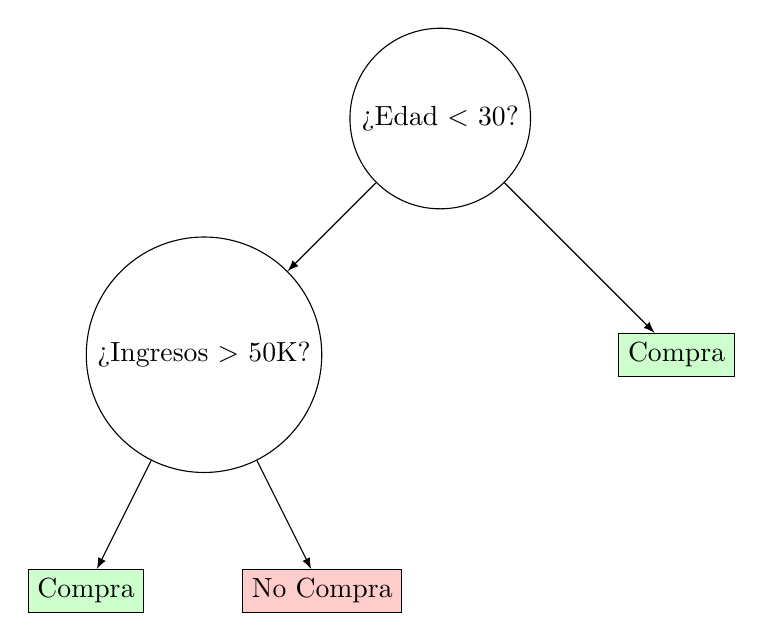
\begin{tikzpicture}[level distance=3cm,
      level 1/.style={sibling distance=6cm},
      level 2/.style={sibling distance=3cm},
      edge from parent/.style={draw,-latex}]
    \node[draw, circle]{¿Edad $<$ 30?}
        child { node[draw, circle]{¿Ingresos $>$ 50K?}
            child { node[draw, rectangle, fill=green!20]{Compra}}
            child { node[draw, rectangle, fill=red!20]{No Compra}}
        }
        child { node[draw, rectangle, fill=green!20]{Compra}};
    \end{tikzpicture}
    \caption{Ejemplo de árbol de decisión para predecir compras}
\end{figure}

\subsection{Sobreajuste y Regularización}

Los árboles de decisión tienden a sobreajustarse si se les permite crecer sin restricciones. Para evitarlo, se utilizan técnicas de regularización:

\begin{itemize}
    \item \textbf{Poda del Árbol:} Remover ramas que aportan poco poder predictivo.
    \item \textbf{Limitación de la Profundidad:} Establecer una profundidad máxima para el árbol.
    \item \textbf{Número Mínimo de Muestras en una Hoja:} Evitar hojas con muy pocas muestras.
\end{itemize}

\subsection{Métodos de Ensamble}

Los \textbf{métodos de ensamble} combinan múltiples modelos base para mejorar el rendimiento general. Se basan en el principio de que una combinación de modelos puede producir resultados más robustos y precisos.

\subsubsection{Bagging (Bootstrap Aggregating)}

\textbf{Bagging} reduce la varianza al promediar múltiples modelos entrenados en subconjuntos de datos obtenidos mediante \textbf{bootstrap} (muestreo con reemplazo).

\paragraph{Algoritmo de Bagging}

\begin{enumerate}
    \item Para $m = 1$ hasta $M$ (número de modelos base):
    \begin{enumerate}
        \item Generar un conjunto de entrenamiento $D_m$ mediante bootstrap de los datos originales.
        \item Entrenar un modelo base $h_m$ en $D_m$.
    \end{enumerate}
    \item Para predicciones:
    \begin{itemize}
        \item \textbf{Clasificación:} Votación mayoritaria entre los modelos $h_m$.
        \item \textbf{Regresión:} Promedio de las predicciones de los modelos $h_m$.
    \end{itemize}
\end{enumerate}

\subsubsection{Random Forest}

El \textbf{Random Forest} es una extensión del bagging que introduce aleatoriedad adicional al seleccionar aleatoriamente un subconjunto de características en cada división.

\paragraph{Características Clave}

\begin{itemize}
    \item Cada árbol se entrena con una muestra bootstrap del conjunto de datos.
    \item En cada nodo, se consideran solo un número aleatorio de características para la división.
\end{itemize}

\subsubsection{Boosting}

El \textbf{Boosting} construye modelos base secuencialmente, donde cada modelo intenta corregir los errores de los anteriores.

\paragraph{AdaBoost (Adaptive Boosting)}

\begin{enumerate}
    \item Inicializar los pesos de las muestras uniformemente.
    \item Para $m = 1$ hasta $M$:
    \begin{enumerate}
        \item Entrenar un modelo base $h_m$ usando los pesos actuales.
        \item Calcular el error ponderado $\epsilon_m$ del modelo.
        \item Calcular el peso del modelo $\alpha_m = \ln\left(\frac{1 - \epsilon_m}{\epsilon_m}\right)$.
        \item Actualizar los pesos de las muestras:
        \[
        w_i \leftarrow w_i \times \exp\left(\alpha_m \times I(y_i \neq h_m(x_i))\right)
        \]
        donde $I$ es la función indicadora.
        \item Normalizar los pesos para que sumen 1.
    \end{enumerate}
    \item La predicción final es:
    \[
    H(x) = \text{sign}\left(\sum_{m=1}^{M} \alpha_m h_m(x)\right)
    \]
\end{enumerate}

\paragraph{Gradient Boosting}

El \textbf{Gradient Boosting} construye modelos secuencialmente optimizando una función de pérdida arbitraria mediante descenso de gradiente.

\begin{enumerate}
    \item Inicializar el modelo con una constante:
    \[
    F_0(x) = \arg\min_{\gamma} \sum_{i=1}^{n} L(y_i, \gamma)
    \]
    \item Para $m = 1$ hasta $M$:
    \begin{enumerate}
        \item Calcular los residuos:
        \[
        r_{i,m} = -\left[ \frac{\partial L(y_i, F_{m-1}(x_i))}{\partial F_{m-1}(x_i)} \right]
        \]
        \item Entrenar un modelo base $h_m$ para predecir los residuos $r_{i,m}$.
        \item Actualizar el modelo:
        \[
        F_m(x) = F_{m-1}(x) + \nu h_m(x)
        \]
        donde $\nu$ es la tasa de aprendizaje.
    \end{enumerate}
\end{enumerate}

\subsection{Comparación entre Bagging y Boosting}

\begin{itemize}
    \item \textbf{Bagging:}
    \begin{itemize}
        \item Reduce la varianza.
        \item Los modelos base son entrenados independientemente.
        \item Bueno para modelos de alto sesgo.
    \end{itemize}
    \item \textbf{Boosting:}
    \begin{itemize}
        \item Reduce el sesgo.
        \item Los modelos base se entrenan secuencialmente.
        \item Bueno para modelos de baja varianza.
    \end{itemize}
\end{itemize}

\subsection{Ventajas y Desventajas}

\textbf{Árboles de Decisión:}

\begin{itemize}
    \item \textbf{Ventajas:}
    \begin{itemize}
        \item Fácil de interpretar y visualizar.
        \item Maneja tanto datos numéricos como categóricos.
        \item Requiere poco preprocesamiento de datos.
    \end{itemize}
    \item \textbf{Desventajas:}
    \begin{itemize}
        \item Propensos al sobreajuste.
        \item Sensibles a pequeñas variaciones en los datos.
    \end{itemize}
\end{itemize}

\textbf{Métodos de Ensamble:}

\begin{itemize}
    \item \textbf{Ventajas:}
    \begin{itemize}
        \item Mejoran la precisión del modelo.
        \item Reducen la varianza y/o el sesgo.
        \item Son más robustos al sobreajuste que los modelos individuales.
    \end{itemize}
    \item \textbf{Desventajas:}
    \begin{itemize}
        \item Menos interpretables que los árboles individuales.
        \item Mayor complejidad computacional.
    \end{itemize}
\end{itemize}

\subsection{Consideraciones Prácticas}

\begin{itemize}
    \item \textbf{Selección de Hiperparámetros:} Es importante ajustar parámetros como la profundidad de los árboles, el número de estimadores y la tasa de aprendizaje en boosting.
    \item \textbf{Balance entre Sesgo y Varianza:} Entender las características del problema para elegir entre bagging y boosting.
    \item \textbf{Escalabilidad:} Los métodos de ensamble pueden ser computacionalmente intensivos; considerar el uso de paralelización.
\end{itemize}

\subsection{Resumen}

Los árboles de decisión son modelos intuitivos y fáciles de interpretar, pero pueden sufrir de sobreajuste. Los métodos de ensamble como bagging y boosting combinan múltiples modelos para mejorar el rendimiento y reducir problemas de sesgo y varianza. La elección del método adecuado depende de las características del problema y los datos disponibles.


\newpage
\section{Clase 4: Máquinas de Vectores de Soporte (SVM)}

\subsection{Introducción}
Las \textbf{Máquinas de Vectores de Soporte (SVM)} son modelos de aprendizaje supervisado utilizados para tareas de clasificación y regresión. El objetivo principal es encontrar el hiperplano que mejor separa las clases de datos con el \textbf{máximo margen} posible.

\subsection{Conceptos Clave}

\begin{definition}
\textbf{Margen:} Es la distancia entre el hiperplano de separación y los puntos más cercanos de cualquier clase.
\end{definition}

\begin{definition}
\textbf{Vectores de Soporte:} Son los puntos de datos que están más cercanos al hiperplano y que definen la posición y orientación del mismo.
\end{definition}

\subsection{Formulación del Problema}

Para datos separables linealmente, buscamos un hiperplano definido por $\mathbf{w}$ y $b$ que satisfaga:

\[
\begin{cases}
\mathbf{w} \cdot \mathbf{x_i} + b \geq +1 & \text{si } y_i = +1 \\
\mathbf{w} \cdot \mathbf{x_i} + b \leq -1 & \text{si } y_i = -1
\end{cases}
\]

El margen se maximiza minimizando $\|\mathbf{w}\|$, lo que conduce al siguiente problema de optimización:

\[
\min_{\mathbf{w}, b} \frac{1}{2} \|\mathbf{w}\|^2 \quad \text{sujeto a } y_i (\mathbf{w} \cdot \mathbf{x_i} + b) \geq 1
\]

\subsection{Función de Costo Hinge y Regularización}

Para datos no separables, introducimos variables de holgura $\xi_i$ y el parámetro de regularización $C$:

\[
\min_{\mathbf{w}, b} \frac{1}{2} \|\mathbf{w}\|^2 + C \sum_{i=1}^{n} \xi_i \quad \text{sujeto a } y_i (\mathbf{w} \cdot \mathbf{x_i} + b) \geq 1 - \xi_i, \quad \xi_i \geq 0
\]

La \textbf{función de costo hinge} es:

\[
L = \sum_{i=1}^{n} \max(0, 1 - y_i (\mathbf{w} \cdot \mathbf{x_i} + b))
\]

\subsection{Ejemplo Visual de SVM Lineal}

\begin{figure}[h!]
    \centering
    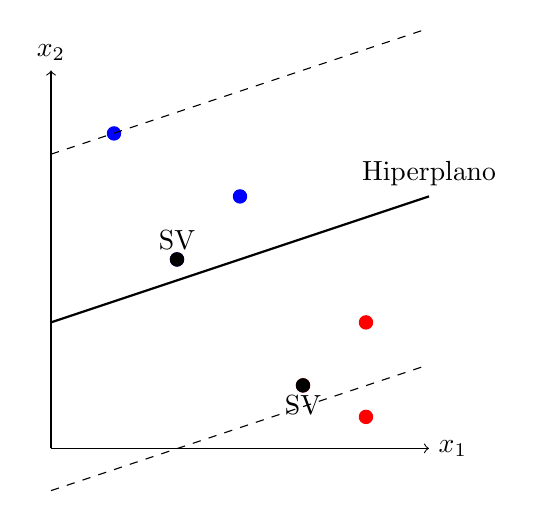
\begin{tikzpicture}[scale=0.8]
    \draw[->] (0,0) -- (6,0) node[right] {$x_1$};
    \draw[->] (0,0) -- (0,6) node[above] {$x_2$};
    % Datos de clase +1
    \filldraw[blue] (1,5) circle (3pt);
    \filldraw[blue] (2,3) circle (3pt);
    \filldraw[blue] (3,4) circle (3pt);
    % Datos de clase -1
    \filldraw[red] (4,1) circle (3pt);
    \filldraw[red] (5,2) circle (3pt);
    \filldraw[red] (5,0.5) circle (3pt);
    % Hiperplano
    \draw[thick] (0,2) -- (6,4) node[above] {Hiperplano};
    % Márgenes
    \draw[dashed] (0,-0.67) -- (6,1.33);
    \draw[dashed] (0,4.67) -- (6,6.67);
    % Vectores de soporte
    \filldraw[black] (2,3) circle (3pt) node[above] {SV};
    \filldraw[black] (4,1) circle (3pt) node[below] {SV};
    \end{tikzpicture}
    \caption{Máxima separación con SVM lineal}
\end{figure}

\subsection{Kernelización}

Para problemas no linealmente separables, utilizamos \textbf{kernels} para transformar los datos a un espacio de mayor dimensión donde sean separables.
\subsubsection{Ejemplo del Kernel RBF}

El \textbf{kernel de base radial (RBF)} se define como:

\[
k(\mathbf{x_i}, \mathbf{x_j}) = \exp(-\gamma \|\mathbf{x_i} - \mathbf{x_j}\|^2)
\]

Donde $\gamma$ es un parámetro que controla el alcance de la influencia de cada punto de entrenamiento.

\begin{figure}[h!]
    \centering
    % Insertar la imagen llamada idea.png
    \includegraphics[width=0.5\textwidth]{idea.png}
    \caption{Transformación de datos con kernel RBF}
\end{figure}

En este ejemplo, los datos que no son separables linealmente en el espacio original se transforman a un espacio de mayor dimensión donde sí lo son.


\subsection{Selección de Hiperparámetros}

\begin{itemize}
    \item \textbf{Parámetro $C$:} Controla la penalización por errores de clasificación.
    \begin{itemize}
        \item $C$ grande: Menos tolerante a errores, margen más pequeño.
        \item $C$ pequeño: Más tolerante a errores, margen más amplio.
    \end{itemize}
    \item \textbf{Parámetro $\gamma$ (en kernel RBF):} Controla la influencia de los puntos de datos individuales.
    \begin{itemize}
        \item $\gamma$ grande: Alcance corto, puede llevar a sobreajuste.
        \item $\gamma$ pequeño: Alcance amplio, puede llevar a subajuste.
    \end{itemize}
\end{itemize}

\subsection{Ejemplo Práctico con SVM}

Supongamos un conjunto de datos donde las clases no son separables linealmente. Al aplicar un kernel RBF, podemos transformar los datos a un espacio de mayor dimensión donde una SVM puede encontrar un hiperplano que las separe.

\subsection{Ventajas y Desventajas}

\textbf{Ventajas:}
\begin{itemize}
    \item Efectivo en espacios de alta dimensionalidad.
    \item Funciona bien cuando el número de dimensiones es mayor que el número de muestras.
    \item Versátil gracias al uso de diferentes kernels.
\end{itemize}

\textbf{Desventajas:}
\begin{itemize}
    \item No es eficiente en conjuntos de datos muy grandes.
    \item Requiere preprocesamiento y ajuste cuidadoso de hiperparámetros.
    \item Difícil de interpretar comparado con modelos más simples.
\end{itemize}

\subsection{Consideraciones Prácticas}

\begin{itemize}
    \item \textbf{Escalado de Características:} Es esencial escalar las características antes de entrenar una SVM.
    \item \textbf{Ajuste de Hiperparámetros:} Utilizar técnicas como la validación cruzada para encontrar los mejores valores de $C$ y $\gamma$.
\end{itemize}


\section{Clase 5: The Bias-Variance Tradeoff}

\subsection{Descomposición del Error de Test}

El error de predicción puede descomponerse en tres componentes principales:

\[
\text{Error} = \text{Bias}^2 + \text{Variance} + \text{Noise}
\]

\subsubsection{Sesgo (\textit{Bias})}
El \textbf{sesgo} mide la diferencia sistemática entre la predicción promedio del modelo y el valor verdadero:
\[
\text{Bias}^2(x) = \left( \mathbb{E}[\hat{f}(x)] - f(x) \right)^2
\]
El sesgo es el principal contribuyente al error en modelos subajustados (\textit{underfitting}).

\subsubsection{Varianza (\textit{Variance})}
La \textbf{varianza} mide cuánto varían las predicciones para un punto de datos dado debido a diferentes realizaciones del modelo:
\[
\text{Variance}(x) = \mathbb{E}\left[\left( \hat{f}(x) - \mathbb{E}[\hat{f}(x)] \right)^2 \right]
\]
Los modelos sobreajustados (\textit{overfitting}) tienden a tener errores altos debido a la varianza.

\subsection{Ejemplos del Tradeoff Sesgo-Varianza}
\subsubsection{LOESS Regression}
En la regresión \textbf{LOESS}, el tradeoff sesgo-varianza se controla mediante el parámetro de suavización.

\subsubsection{K-Nearest Neighbors (KNN)}
En \textbf{KNN}, el parámetro \(K\) controla el tradeoff. Valores pequeños de \(K\) implican alta varianza, mientras que valores grandes conllevan alto sesgo.
\newpage
\section{Clase 6: Selección de Modelos}

\subsection{Evaluación}
\begin{itemize}
    \item Para saber si podemos \textit{confiar} en nuestro método o sistema, necesitamos evaluarlo.
    \item Si no podemos medirlo, no podemos mejorarlo.
    \item Selección de modelo: elegir entre diferentes modelos usando un enfoque basado en datos.
    \item Convencer a otros de que el trabajo de uno es significativo.
\end{itemize}

\subsubsection{Diseño de sistemas de machine learning}

\begin{itemize}
    \item Simplemente correr el algoritmo favorito de uno, generalmente no es una buena manera de comenzar.
    \item Considere el problema en general:
    \begin{itemize}
        \item ¿Queremos entender los fenómenos o realizar un modelo caja negra?
        \item ¿Cómo definir y medir el éxito? ¿Hay costos involucrados?
        \item ¿Se tienen los datos correctos? ¿Cómo puedes mejorarlo?
    \end{itemize}
    \item Construir prototipos desde el principio para evaluar los cambios a lo largo del tiempo.
    \item Analizar los errores del modelo que uno está construyendo (entrenando):
    \begin{itemize}
        \item ¿Debería recopilar más datos, o datos adicionales?
        \item ¿Debería reformularse la tarea?
    \end{itemize}
    \item Deuda técnica: compensación de creación-mantenimiento:
    \begin{itemize}
        \item Los sistemas de aprendizaje automático muy complejos son difíciles/imposibles de poner en práctica.
        \item Revisar \textit{Machine Learning: The High Interest Credit Card of Technical Debt} \url{https://storage.googleapis.com/pub-tools-public-publication-data/pdf/43146.pdf}
    \end{itemize}
\end{itemize}

\subsubsection{Evaluaciones en el mundo real}
\begin{itemize}
    \item Evaluar predicciones, pero también cómo mejoraron los resultados \textit{gracias a ellas}.
    \item Feedback loops: las predicciones se introducen en las entradas, como datos nuevos.
    \item La señal que encontró su modelo puede ser solo un artefacto de sus datos sesgados.
    \begin{itemize}
        \item Cuando sea posible, intente \textit{interpretar} lo que su modelo ha aprendido.
        \item Revisar \textit{Why Should I Trust You?} \url{https://www.kdd.org/kdd2016/papers/files/rfp0573-ribeiroA.pdf} por Marco Ribeiro et al.
    \end{itemize}
\end{itemize}

\subsubsection{Técnicas de estimación de desempeño}
\begin{itemize}
    \item No tenemos acceso a futuras observaciones.
    \item Evaluar modelos \textit{como si estuvieran prediciendo el futuro}.
    \item Reserve datos para una evaluación objetiva.
\end{itemize}

\subsection{The holdout (partición simple train-test)}
Ya hemos visto la forma más básica de evaluación.

\subsubsection{Cross-validation}
\begin{itemize}
    \item ¿Qué pasa si una división aleatoria produce diferentes modelos (y scores) que otra?
    \item Reduzca el sesgo probando en cada punto exactamente una vez.
    \item \textit{Validación cruzada de k-dobladas} o \textit{k-fold cross-validation} (CV): particionar (split) aleatoriamente en $k$ partes del mismo tamaño, llamadas \textit{folds}. Supongamos $k=5$:
    \begin{itemize}
        \item Primero, el fold 1 es el conjunto de prueba, y los folds 2-5 comprenden el conjunto de entrenamiento.
        \item Luego, el fold 2 es el conjunto de prueba, los folds 1,3,4,5 comprenden el conjunto de entrenamiento.
        \item Calcule las $k$ puntuaciones de evaluación, agregue después (por ejemplo, tome la media).
    \end{itemize}
\end{itemize}

\subsubsection{Beneficios y desventajas de cross-validation}
\begin{itemize}
    \item Más robusto: cada ejemplo de entrenamiento estará en un conjunto de prueba exactamente una vez.
    \begin{itemize}
        \item El modelo se evalúa en todas las muestras, debe funcionar bien en todas.
        \item En una partición train-test, podemos tener:
        \begin{itemize}
            \item `suerte': todos los ejemplos sencillos están en el conjunto de prueba.
            \item `desafortunado': todos los ejemplos difíciles están en el conjunto de prueba.
        \end{itemize}
    \end{itemize}
    \item Muestra cuán \textit{sensible} es el modelo al conjunto de entrenamiento exacto.
    \item Mejor estimación del rendimiento real.
\end{itemize}

\subsection{Matriz de confusión y métricas de clasificación}

La \textbf{matriz de confusión} es una herramienta útil para evaluar el rendimiento de un clasificador. Para una clasificación binaria, la matriz de confusión se organiza de la siguiente manera:

\begin{center}
\begin{tabular}{|c|c|c|}
 \hline
   & Predicción Positiva & Predicción Negativa \\
 \hline
 Clase Positiva & Verdaderos Positivos (TP) & Falsos Negativos (FN) \\
 \hline
 Clase Negativa & Falsos Positivos (FP) & Verdaderos Negativos (TN) \\
 \hline
\end{tabular}
\end{center}

A partir de esta matriz, podemos calcular diversas métricas importantes:

\subsubsection{Precisión (Accuracy)}
La \textbf{precisión} es la proporción de predicciones correctas entre el total de predicciones realizadas.

\[
\text{Accuracy} = \frac{TP + TN}{TP + TN + FP + FN}
\]

\subsubsection{Precision}
La \textbf{precision} se utiliza para medir la calidad de las predicciones positivas. Indica cuántas de las predicciones positivas fueron correctas.

\[
\text{Precision} = \frac{TP}{TP + FP}
\]

\subsubsection{Recall}
El \textbf{recall} o \textit{sensibilidad} mide cuántas de las muestras positivas reales fueron correctamente identificadas.

\[
\text{Recall} = \frac{TP}{TP + FN}
\]

\subsubsection{F1-Score}
El \textbf{F1-score} es la media armónica entre la precision y el recall. Es útil cuando buscamos un equilibrio entre ambos.

\[
\text{F1} = 2 \cdot \frac{\text{Precision} \cdot \text{Recall}}{\text{Precision} + \text{Recall}}
\]

\subsubsection{Área bajo la curva ROC (AUC)}
El \textbf{AUC} es una métrica basada en la curva ROC que mide la capacidad del modelo para separar correctamente las clases. Es especialmente útil en conjuntos de datos desbalanceados, ya que es insensible al desbalanceo de clases.

\subsection{Métricas para Regresión}

En los problemas de regresión, las métricas comunes incluyen:

\subsubsection{Error cuadrático medio (MSE)}
El \textbf{Mean Squared Error (MSE)} mide el promedio de los errores al cuadrado entre las predicciones y los valores verdaderos.

\[
\text{MSE} = \frac{1}{n} \sum_{i=1}^{n} (y_i - \hat{y_i})^2
\]

\subsubsection{Error absoluto medio (MAE)}
El \textbf{Mean Absolute Error (MAE)} mide el promedio de los errores absolutos entre las predicciones y los valores verdaderos, menos sensible a los valores atípicos.

\[
\text{MAE} = \frac{1}{n} \sum_{i=1}^{n} |y_i - \hat{y_i}|
\]

\subsubsection{Coeficiente de determinación ($R^2$)}
El \textbf{R-squared} mide la proporción de la varianza explicada por el modelo en comparación con la varianza total. Tiene un valor entre 0 y 1, y puede ser negativo si el modelo es peor que predecir la media.

\[
R^2 = 1 - \frac{\sum_{i=1}^{n} (y_i - \hat{y_i})^2}{\sum_{i=1}^{n} (y_i - \bar{y})^2}
\]
\newpage

\subsection{Resumen I}

\subsubsection{k-fold Cross-validation}
\begin{itemize}
    \item Elija $k$ dependiendo de la cantidad de datos que tenga.
    \begin{itemize}
        \item $k$ grande es más lento, pero permite más datos de entrenamiento.
        \item 10-fold, 5-fold, 5x2-fold son las opciones más populares.
    \end{itemize}
    \item Utilice siempre la estratificación para la clasificación (especialmente en los casos desbalanceados).
    \item División Train-test y Shuffle-split: útil para grandes conjuntos de datos.
    \item Utilice grouping cuando se quiera generalizar sobre grupos.
\end{itemize}

\subsubsection{Selección de modelo}
\begin{itemize}
    \item No agregue sobre los puntajes de test: aquellos que han visto los datos del test set.
    \item Utilice conjuntos de validación para elegir primero algoritmos/hiperparámetros.
\end{itemize}

\subsubsection{Optimización}
\begin{itemize}
    \item \textbf{Grid Search}: exhaustivo pero simple.
    \item \textbf{Random Search}: escala mejor.
\end{itemize}

\subsection{Resumen II}
\begin{itemize}
    \item Los datos del mundo real a menudo están desbalanceados.
    \item Los falsos positivos pueden ser mucho peores que los falsos negativos (o viceversa).
    \item Clasificación binaria:
    \begin{itemize}
        \item Seleccione métricas que puedan distinguir diferentes tipos de errores (precision, recall, F1-score, AUC,...).
        \item Calibre los umbrales de decisión para la tarea en cuestión.
        \item Curvas de Precision-Recall y ROC: elija el mejor umbral o tome el área debajo de la curva.
    \end{itemize}
    \item Clasificación multiclase:
    \begin{itemize}
        \item Promedio Macro/Micro/weighted de puntajes por clase (one-vs-all).
    \end{itemize}
    \item Regresión:
    \begin{itemize}
        \item (Root) mean squared/absolute error desde 0..Inf.
        \item $R^2$ más fácil de interpretar.
    \end{itemize}
    \item Todas las medidas se pueden utilizar en cross-validation o grid/random search.
    \item Clasificación Cost-sensitive: optimizar para cualquier matriz de costos o función de costos.
\end{itemize}
\newpage

\section{Comparativas}

En esta sección, se comparan los diferentes algoritmos estudiados en las clases anteriores, evaluando sus principales diferencias, fortalezas, debilidades y casos de uso recomendados. A continuación, se presentan tablas comparativas que resumen esta información.
\begin{table}[h!]
\centering
\resizebox{\textwidth}{!}{
\begin{tabular}{@{}lccc@{}}
\toprule
\textbf{Característica} & \textbf{kNN} & \textbf{Árboles de Decisión} & \textbf{SVM} \\ \midrule
\textbf{Tipo de Modelo} & No paramétrico & Paramétrico & Paramétrico \\
\textbf{Aprendizaje} & Instancia & Basado en reglas & Margen máximo \\
\textbf{Uso} & Clasificación/Regresión & Clasificación/Regresión & Clasificación/Regresión \\
\textbf{Interpretabilidad} & Baja & Alta & Baja \\
\textbf{Escalabilidad} & Baja & Media & Baja \\
\textbf{Manejo de Datos} & Datos pequeños & Datos medianos & Datos pequeños \\
\textbf{Sensibilidad a Dimensionalidad} & Alta & Media & Media \\
\textbf{Resistencia al Overfitting} & Baja (k pequeño) & Baja (árbol profundo) & Alta \\
\textbf{Principales Hiperparámetros} & $k$, distancia & Profundidad, criterios de división & $C$, kernel, $\gamma$ \\
\textbf{Fortalezas} & Fácil de implementar & Fácil de interpretar & Maneja datos no lineales \\
\textbf{Debilidades} & Lento en predicción & Sobreajuste si no se poda & Requiere ajuste de hiperparámetros \\
\bottomrule
\end{tabular}
}
\caption{Comparativa de otros algoritmos.}
\end{table}

\begin{table}[h!]
\centering
\resizebox{\textwidth}{!}{
\begin{tabular}{lcccc}
\toprule
\textbf{Característica} & \textbf{Bagging} & \textbf{Random Forest} & \textbf{AdaBoost} & \textbf{Gradient Boosting} \\ \midrule
\textbf{Tipo de Modelo} & Ensamble & Ensamble & Ensamble & Ensamble \\
\textbf{Aprendizaje} & Basado en ensamble & Basado en ensamble & Basado en ensamble & Basado en ensamble \\
\textbf{Uso} & Clasificación/Regresión & Clasificación/Regresión & Clasificación & Clasificación/Regresión \\
\textbf{Interpretabilidad} & Media & Media & Baja & Baja \\
\textbf{Escalabilidad} & Baja & Media & Baja & Baja \\
\textbf{Manejo de Datos} & Datos medianos & Datos grandes & Datos medianos & Datos medianos \\
\textbf{Sensibilidad a Dimensionalidad} & Media & Media & Media & Media \\
\textbf{Resistencia al Overfitting} & Alta & Alta & Media & Media \\
\textbf{Principales Hiperparámetros} & Número de modelos & Número de árboles, profundidad & Número de modelos, tasa de aprendizaje & Número de modelos, tasa de aprendizaje \\
\textbf{Fortalezas} & Reduce varianza & Reduce varianza & Mejora precisión & Mejora precisión \\
\textbf{Debilidades} & Requiere recursos & Complejo & Sensible al ruido & Sensible al ruido \\
\bottomrule
\end{tabular}
}
\caption{Comparativa de algoritmos de ensamble.}
\end{table}



\subsection{Casos de Uso y Selección de Algoritmo}

En la siguiente tabla se resumen las situaciones en las que es más adecuado utilizar cada algoritmo, según las características del problema y los datos disponibles.

\begin{table}[h!]
\centering
\begin{tabular}{@{}ll@{}}
\toprule
\textbf{Algoritmo} & \textbf{Casos de Uso Recomendados} \\ \midrule
kNN & \begin{tabular}[c]{@{}l@{}}- Problemas con conjuntos de datos pequeños.\\ - Cuando se requiere un modelo rápido de entrenar.\\ - Cuando no se necesita interpretabilidad.\end{tabular} \\
Árboles de Decisión & \begin{tabular}[c]{@{}l@{}}- Cuando se requiere interpretabilidad.\\ - Datos con relaciones no lineales.\\ - Problemas de clasificación y regresión.\end{tabular} \\
Bagging & \begin{tabular}[c]{@{}l@{}}- Reducir varianza de modelos inestables.\\ - Cuando se dispone de recursos computacionales.\\ - Mejorar precisión en datos medianos.\end{tabular} \\
Random Forest & \begin{tabular}[c]{@{}l@{}}- Conjuntos de datos grandes.\\ - Problemas con muchas características.\\ - Necesidad de reducir varianza y manejar overfitting.\end{tabular} \\
AdaBoost & \begin{tabular}[c]{@{}l@{}}- Cuando se necesita mejorar el rendimiento de clasificadores débiles.\\ - Datos con ruido moderado.\\ - Problemas de clasificación binaria.\end{tabular} \\
Gradient Boosting & \begin{tabular}[c]{@{}l@{}}- Alta precisión en clasificación y regresión.\\ - Datos con patrones complejos.\\ - Cuando se pueden ajustar hiperparámetros cuidadosamente.\end{tabular} \\
SVM & \begin{tabular}[c]{@{}l@{}}- Datos de alta dimensionalidad.\\ - Problemas de clasificación con fronteras complejas.\\ - Cuando el número de muestras es menor que el de características.\end{tabular} \\
\bottomrule
\end{tabular}
\caption{Recomendaciones para la selección de algoritmos según el caso de uso.}
\end{table}

\subsection{Principales Diferencias entre los Algoritmos}

\begin{itemize}
    \item \textbf{kNN vs. Árboles de Decisión:} kNN es un método basado en instancias que requiere almacenar todo el conjunto de datos y es sensible a la dimensionalidad, mientras que los árboles de decisión generan un modelo interpretable y manejan mejor características irrelevantes.

    \item \textbf{Ensamble (Bagging, Random Forest) vs. Modelos Simples:} Los ensambles combinan múltiples modelos para reducir la varianza y mejorar la precisión, a costa de una mayor complejidad y menor interpretabilidad.

    \item \textbf{Boosting (AdaBoost, Gradient Boosting) vs. Bagging:} Mientras que Bagging busca reducir la varianza mediante la combinación de modelos independientes, Boosting reduce el sesgo construyendo secuencialmente modelos que corrigen los errores de los anteriores.

    \item \textbf{SVM vs. Otros Algoritmos:} Las SVM son eficaces en espacios de alta dimensionalidad y pueden manejar relaciones no lineales mediante kernels, pero requieren un ajuste cuidadoso de hiperparámetros y pueden ser computacionalmente costosas con grandes conjuntos de datos.
\end{itemize}

\subsection{Evaluación para la Selección de Algoritmo}

Al seleccionar un algoritmo, se deben considerar los siguientes aspectos:

\begin{itemize}
    \item \textbf{Tamaño y Dimensionalidad de los Datos:} Algoritmos como kNN y SVM pueden no escalar bien con conjuntos de datos muy grandes.

    \item \textbf{Interpretabilidad:} Si es crucial entender las decisiones del modelo, los árboles de decisión son preferibles.

    \item \textbf{Recursos Computacionales:} Ensambles y SVM pueden requerir más tiempo y recursos para entrenar y predecir.

    \item \textbf{Rendimiento y Precisión:} Ensambles como Random Forest y Gradient Boosting suelen ofrecer mayor precisión a costa de interpretabilidad.

    \item \textbf{Presencia de Ruido y Outliers:} Algoritmos como AdaBoost pueden ser sensibles al ruido, mientras que Random Forest es más robusto.

    \item \textbf{Necesidad de Ajuste de Hiperparámetros:} Modelos como SVM y Gradient Boosting requieren un ajuste cuidadoso para obtener un buen rendimiento.
\end{itemize}

\subsection{Conclusión}

La elección del algoritmo adecuado depende de múltiples factores, incluyendo las características del conjunto de datos, los recursos disponibles y los objetivos específicos del problema. Las tablas y comparativas presentadas sirven como guía para orientar esta selección, pero es recomendable realizar pruebas y validaciones cruzadas para determinar el mejor modelo para cada caso particular.


\end{document}
